\documentclass{fkssolpub}

\usepackage[czech]{babel}
\usepackage{fontspec}
\usepackage{fkssugar}
\usepackage{amsmath}
\usepackage{graphicx}

\author{Ondřej Sedláček}
\school{Gymnázium Oty Pavla} 
\series{3p}
\problem{3} 

\begin{document}

\begin{figure}[h!]
	\centering
	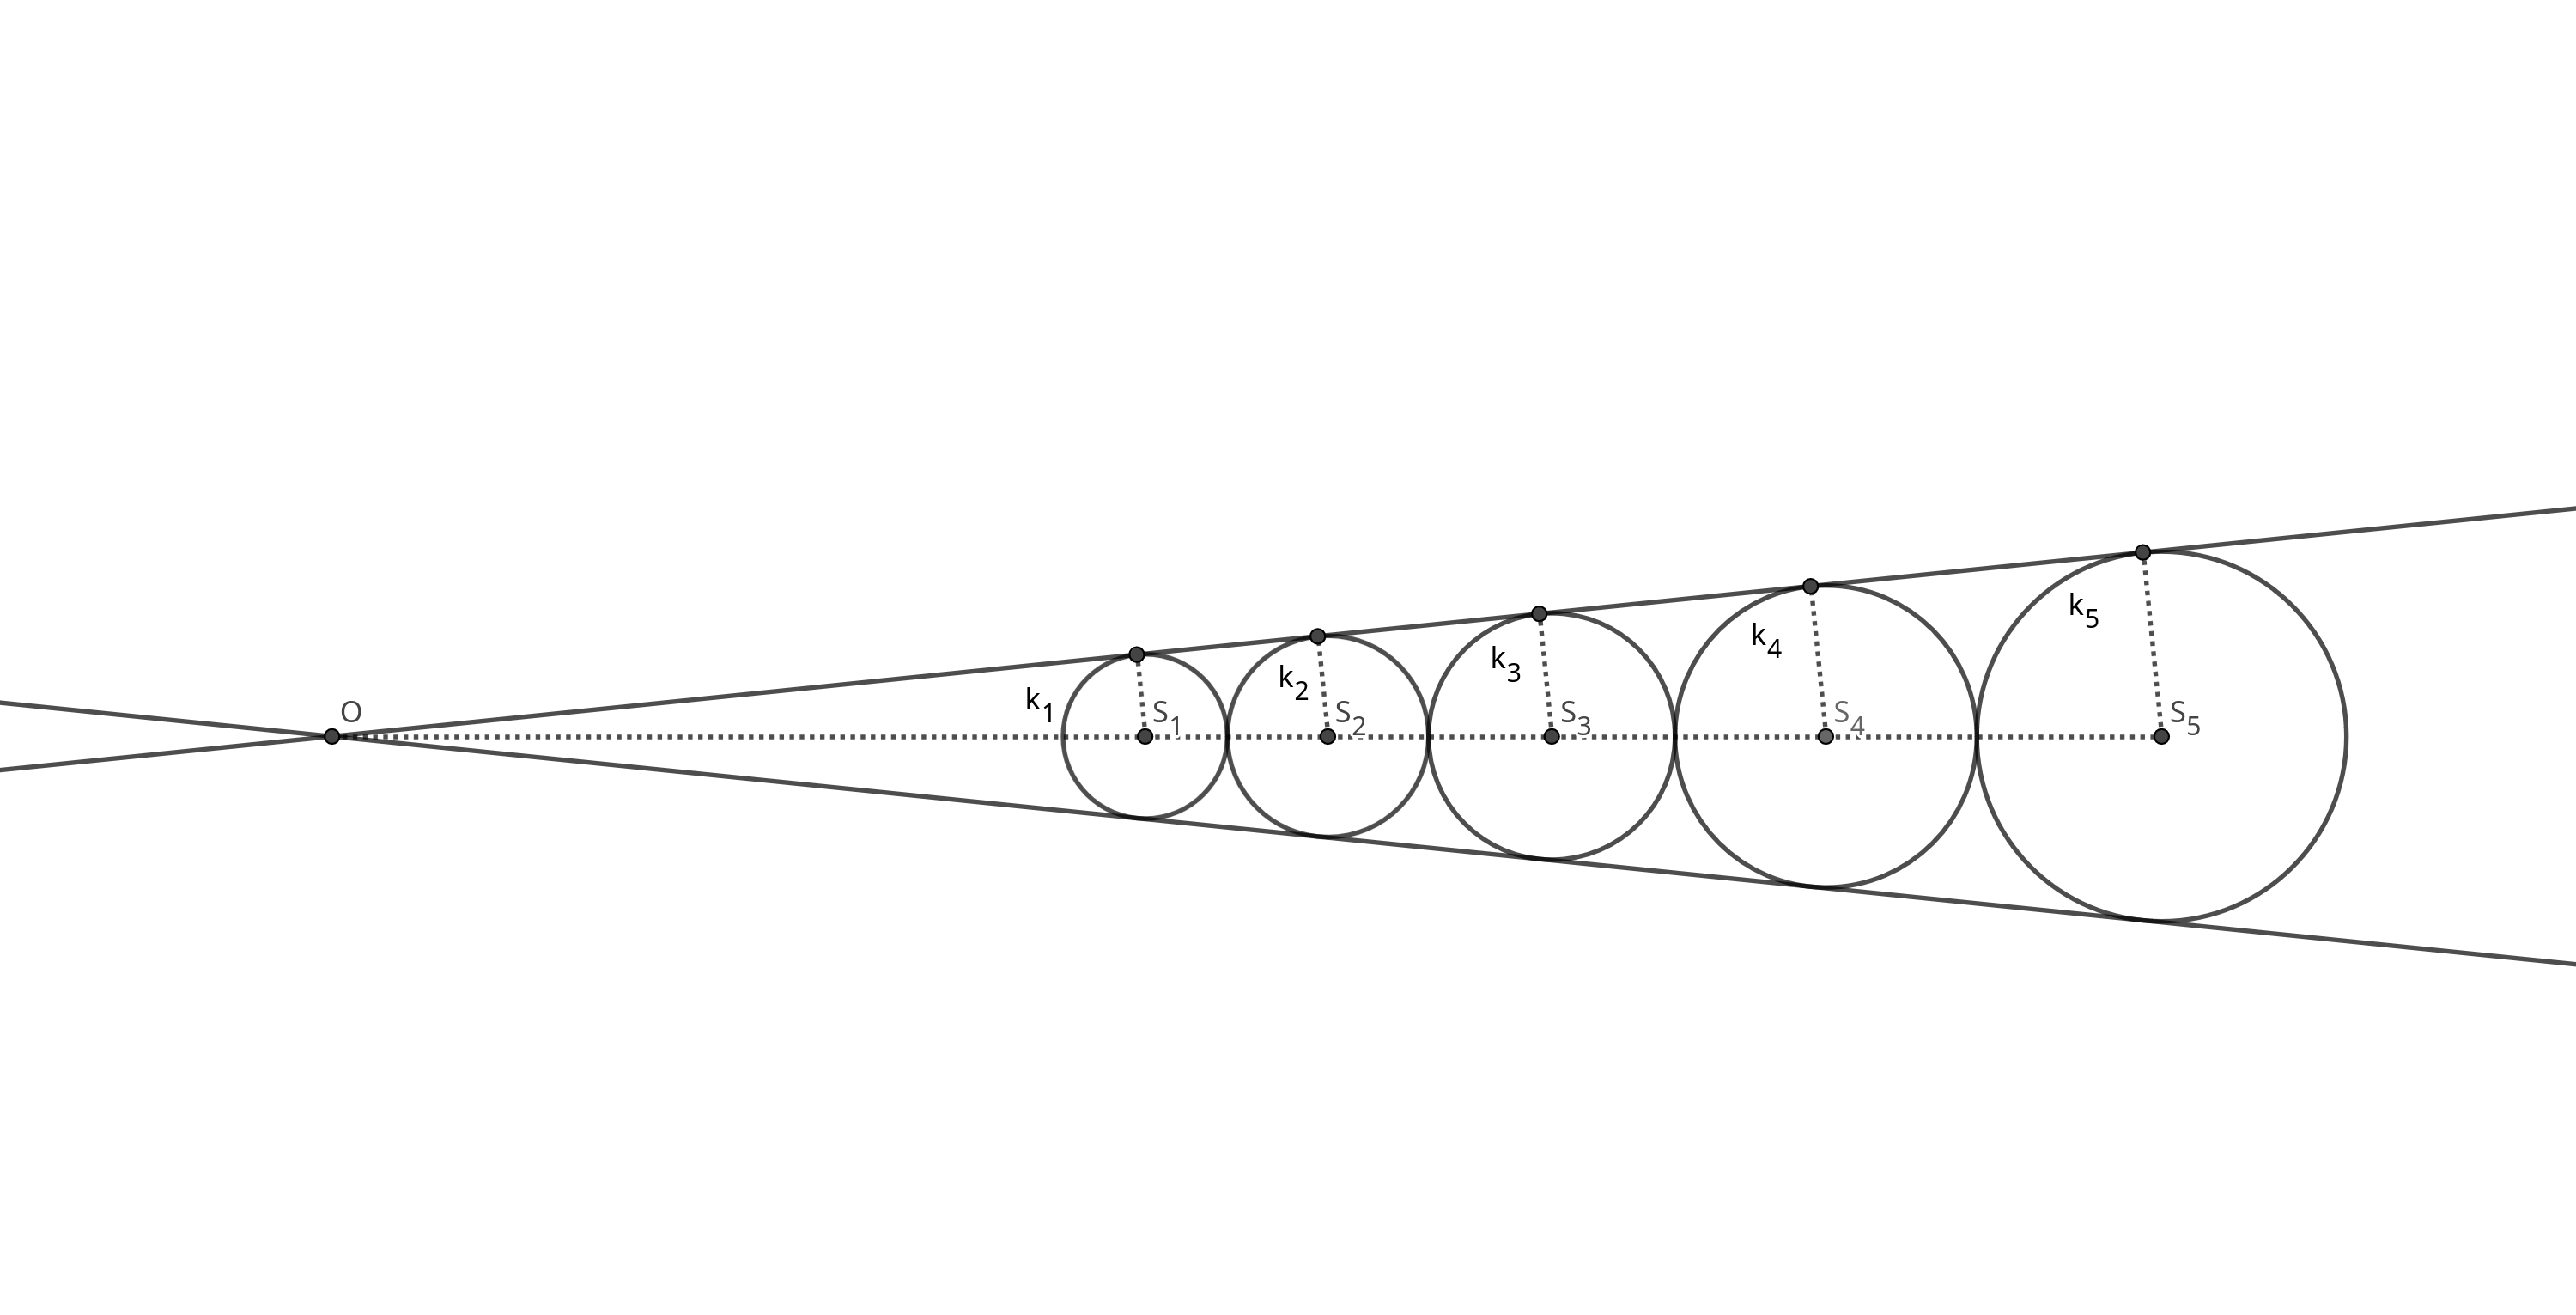
\includegraphics[width=\textwidth]{3-fig.png}
	\caption{Konstrukce ze zadání}
\end{figure}

Na obrázku si můžeme všimnout toho, že všechny narýsované kružnice
jsou si navzájem stejnolehlé se středem $O$ a různými koeficienty.
Mohlo by nás však napadnout hypotéza, jestli když známe koeficient
stejnolehlosti $x$ mezi kružnicemi $k_1$ a $k_2$, jestli mezi
kružnicemi $k_1$ a $k_n$ koeficient $x^{n - 1}$. To můžeme
dokázat indukcí.

Budeme tedy předpokládat, že platí následující rovnosti:

\[
	r_n = x^{n - 1} r_1
\]
\[
	x^{n - 1}(l + r_1) = l + 2r_1 + ... + 2r_{n - 1} + r_n
\]

Díky tomu, že $x$ je koeficient mezi kružnicemi $k_1$ a $k_2$,
nutně tedy platí:

\begin{equation}
	x (l + r_1) = l + 2r_1 + x r_1 \ztoho xl = l + 2r_1
	\label{eq:1}
\end{equation}

Pak dokážeme, že indukční předpoklad platí pro všechna
přirozená čísla:

\[
	x^{n - 1}(l + r_1) = l + 2r_1 + ... + 2r_{n - 1} + r_n
\]
\[
	x^{n - 1}(l + r_1) = x^{n - 2}(l + r_1) + r_{n - 1} + r_n
\]
\[
	x^{n - 1}(l + r_1) = x^{n - 2}(l + r_1) + x^{n - 2}r_1 + x^{n - 1}r_1
\]
\[
	x^{n - 1} l = x^{n - 2}(l + 2r_1)
\]

Z rovnice \ref{eq:1} pak dosadíme a dosáhneme rovnosti:

\[
	x^{n - 1} l = x^{n - 1} l
\]

Odtud tedy víme, že koeficient mezi kružnicemi $k_1$ a $k_5$ je:

\[
	x^4 = \frac{18}{8} = \frac{9}{4}
\]

Odkud zjistíme koeficient stejnolehlosti mezi kružnicemi $k_1$ a
$k_3$ a následně určíme poloměr kružnice $k_3$:

\[
	r_3 = x^2 r_1 = 8 \sqrt{\frac{9}{4}} = 12
\]

Poloměr kružnice $k_3$ je tedy 12.

\end{document}
